% Chapter Template

\chapter{Soluciones presentadas} % Main chapter title
\label{cap:soluciones} % Change X to a consecutive number; for referencing this chapter elsewhere, use \ref{ChapterX}

\section{Metodología}

La puntuación final de la competición será calculada mediante una función de pérdida logarítmica, como vimos en el apartado \ref{sec:envio-y-eval}. Al no tener las categorías del conjunto de datos de test debemos delegar el cálculo de la puntuación en Kaggle, que permite enviar hasta cinco predicciones al día. Esto es un obstáculo para hacer pequeñas pruebas e iterar rápido sobre los resultados. Por otra parte, el segundo conjunto de test tiene más de 13000 imágenes, que no son rápidas de cargar en memoria ni de pasar por el modelo que se genere. En determinados casos la evaluación del segundo conjunto de test ha tardado más de 6 horas.

La solución a este problema se ha resuelto usando un subconjunto del conjunto de entrenamiento dedicado solo a la evaluación de modelos. Por otra parte, para el entrenamiento es necesario usar un subconjunto de validación, por lo tanto es necesario dividir el conjunto de entrenamiento original en tres subconjuntos: entrenamiento, validación y test.

La partición se ha realidado dejando un \textbf{60\%} de los datos al conjunto de entrenamiento, un \textbf{20\%} al conjunto de validación y un \textbf{20\%} al conjunto de test.


\subsection{Partición de conjuntos de datos}
La partición del conjunto de datos es una operación delicada. Ya vimos que uno de los problemas del dataset era que la cantidad de imágenes para cada clase era muy variada, teniendo algunas clases un número muy bajo de ejemplos. Si sacamos el 40\% de las imágenes del dataset, podemos estar vaciando una o varias categorías de ejemplos de entrenamiento, haciendo inútil cualquier clasificación de esas clases.

La solución por la que se ha optado es generar un subconjunto del 20\% usando el 20\% de los ejemplos de cada clase, evitando así vaciar alguna de las clases.

\subsection{Evaluación del modelo}

Para una búsqueda más óptima de parámetros y configuraciones el modelo se evaluará contra el grupo de test generado. Una vez se encuentren determinados modelos especialmente interesantes por tener una puntuación máxima local entre aquellos a los que se compara habrá que enviarlo a Kaggle para su evaluación completa.

Enviar el modelo a Kaggle se puede hacer sobre una partición más grande del conjunto de entrenamiento, ya que no es necesario usar un conjunto de test para evaluar, solo uno de validación. Esto permite entrenar el modelo sobre el 80\% de los datos consiguiendo, por lo general, resultados más precisos.

\subsection{Software}

Todos los modelos de redes convolucionales que se van a entrenar en este proyecto serán modelos de 
\section{Idea}
A la hora de afrontar este problema de clasificación de peces es lógico
seguir una estrategia separada en dos pasos: primero buscar si
existe un pez en la foto y luego intentar clasificarlo en una de las 
categorías existentes. 

Para encontrar un pez en la foto es necesario encontrar una serie de
características que puedan ser identificadas con algún pez. La idea de 
la solución parte de esta base. A la hora de clasificar una imagen
primero es necesario encontrar el contenido relevante para ser usado
en la clasificación.

Como ya se comentó al hablar de las redes convolucionales (capítulo \ref{sec:conv-net-arch}),
las arquitecturas encontradas en problemas similares \parencite{krizhevsky2012imagenet}
permiten separar con claridad estas dos etapas mediante el uso de redes convolucionales (CONV) y capas densas (FC).

\section{Arquitectura}

La arquitectura general usada, que luego sufrirá pequeños cambios, es la descrita en la figura~\ref{general-architecture} (Krizhevsky et al.)

\begin{figure}
  \caption{Arquitectura de la red en dos partes}
\label{general-architecture}
  \makebox[\textwidth]{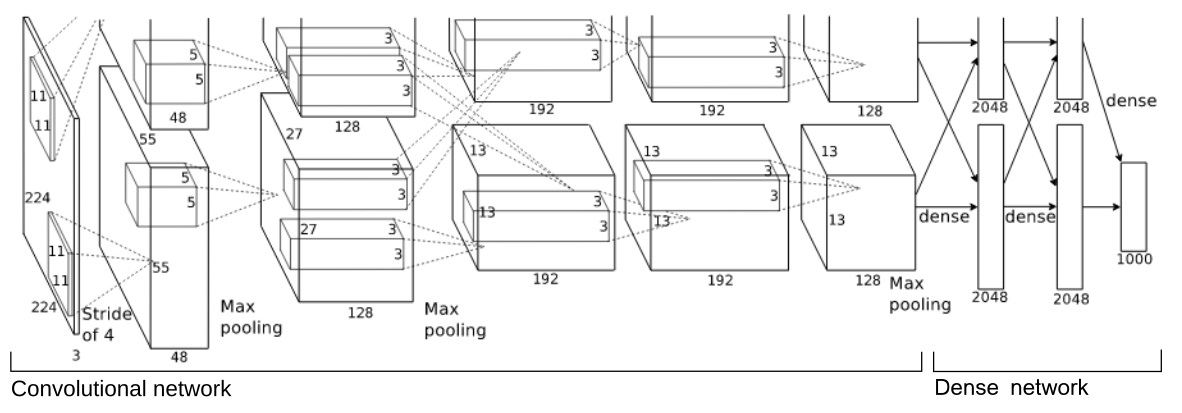
\includegraphics[width=\linewidth]{imagenet-arch}}
\end{figure}

Esta arquitectura usa en su primera parte una red convolucional preentrenada sobre un conjunto de imágenes mucho más generalista, en este caso Imagenet. Al usar una red convolucional preentrenada sobre fotografías tendrá muchas más capacidad para distinguir características de diferentes objetos, además que existen varias categorías de peces en Imagenet, por lo que sabrá diferenciar este tipo de fotografías.


\subsection{Red convolucional}

Como explicamos en el capítulo~\ref{sec:conv-net}, cuando un modelo convolucional recibe una imagen va a devolver $N$ matrices bidimensionales representando el resultado de las aplicación de los $N$ conjuntos de filtros a la imagen inicial. Al ser $N$ matrices bidimensionales también puede considerarse una matriz tridimensional.

Intuitivamente, y haciendo una simplificación, podemos pensar que cada uno de estos filtros representa un mapa de calor de la aparición en la imagen de diferentes características. Por ejemplo, ¿cúanto se parece cada parte de esta imagen a la piel de un pez?.

Hay que tener en cuenta que este modelo convolucional no ha sido entrenado con el conjunto de entrenamiento, si no con el conjunto de entrenamiento de Imagenet. Para lo único que vamos a usar esta red convolucional es para transformar estas imágenes a 

\subsection{Modelo preentrenado}

La arquitectura del artículo original \parencite{krizhevsky2012imagenet} usa capas convolucionales donde alterna filtros de $11\times11$, $5\times5$, y $3\times3$, el cual parece una buena elección para usar como modelo convolucional preentrenado. Sin embargo la aplicación de este trabajo es una competición internacional donde se usarán soluciones \textit{state of the art}. El modelo de la figura \ref{general-architecture} representa el ganador de la edición 2012 de la competición ILSVRC. Un buen punto de partida puede ser mirar los modelos ganadores de años posteriores.

El modelo principal a usar es VGG, desarrollado por el \textit{Visual Geometry Group}, de la Universidad de Oxford. Es un modelo especialmente interesante por su simplicidad, aparte de obtener una de las mejores puntuaciones en ILSVRC 2014.

\section{VGG16}

Una de las principales características de VGG es la idea de que los filtros convolucionales mayores de $3\times3$, como por ejemplo los de $5\times5$ u $11\times11$ pueden ser representados por combinaciones de filtros $3\times3$.

Una de las configuraciones descritas en \parencite{simonyan} se la conoce como VGG16. Usando un total de trece capas CONV con filtros de $3\times3$, cinco capas POOL y tres capas FC (de 4096, 4096 y 1000 salidas), seguido de una función \textit{softmax} (figura \ref{vgg16-arch}), es capaz de mejorar la eficacia del modelo de Krizhevsky. El nombre de esta configuración es VGG16 ya que es la cantidad de capas CONV y FC que posee.

Estamos usando la configuración VGG16 de todas las descritas en su definición original ya que, junto con VGG19, consigue los mejores resultados.

\begin{figure}
  \caption{Arquitectura de VGG}
\label{vgg16-arch}
  \makebox[\textwidth]{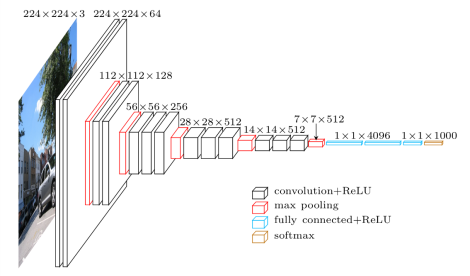
\includegraphics[width=.7\linewidth]{vgg16-arch}}
\end{figure}

\subsection{\textit{Fine-tuning}}

Si observamos la última capa del modelo VGG16, vemos que la salida tiene 1000 elementos. Tiene esta forma ya que ILSVRC consistía en clasificar una imagen entre mil categorías diferentes. Si el problema a resolver consiste en clasificar entre ocho categorías, es lógico modificar esta última capa para que tenga solo ocho salidas.

Al modificar la estructura de la última capa estamos destruyendo pesos y haciendo que muchos de los que ya existían carezcan de sentido. El hecho de que VGG tenga esta separación lógica entre la red convolucional y la red densa (las tres capas FC) hace que se pueda separar el modelo en dos modelos diferentes: uno convolucional, que no habrá cambiado con la adaptación a las ocho categorías, y otro denso, que tendrá que ser reentrenado de nuevo.

Al partir una red en dos partes diferentes hay que tener en cuenta que la segunda parte, la red densa, no recibe como entrada las imágenes, si no la salida de la red convolucional, con todas las transformaciones que esta produce. Es necesario entonces aplicar la red convolucional a todo el conjunto de datos para crear un nuevo conjunto de datos con el que reentrenar la red densa.

Esta técnica de ajustar los paŕametros de un modelo ya conocido para adaptarlo con nuevo conjunto de datos se conoce como \textit{fine-tuning}.

En este punto ya se tienen todas las herramientas necesarias para entrenar un modelo usando VGG16.
\subsection{Batch normalization}
\subsection{Dropout}
\subsection{Data augmentation}
\subsection{Fully convolutional network}

